\documentclass[12pt]{article}

\usepackage{geometry}
\usepackage[utf8]{inputenc}
\usepackage[polish]{babel}
\usepackage{polski}
\usepackage{hyperref}
\usepackage{graphicx}
\usepackage{verbatim}
\usepackage{acronym}
\usepackage{fancyhdr}
\usepackage[usenames]{color}

\hypersetup{
  linkbordercolor={1 1 1},
  urlbordercolor={1 1 1},
  colorlinks=true
}

\pagestyle{fancy}
\cfoot{}
\rfoot{\thepage}

\author{\textbf{Michał Bugno} \and \textbf{Antek Piechnik} \and prowadzący: \textbf{dr inż. Robert Marcjan}}
\title{
Analiza oraz wizualizacja danych meteorologicznych dla wybranych ośrodków narciarskich
\begin{figure*}[h]
  \centerline{
    
\includegraphics[scale=1.0]{images/logo_agh.pdf}
  }
\end{figure*}
}

\begin{document}

\maketitle
\newpage
\tableofcontents
\newpage

\section{Wstęp}
\subsection{Wizja}
Głównym zadaniem projektu jest poznanie struktury
danych typu GIS (geographical information system), jak również analiza oraz
wykorzystanie tego typu danych w wizualizacji danych meteorologicznych. System
docelowo ma za zadanie przedstawienie sytuacji meteorologicznej na podstawie
danych zbieranych na bieżąco jak również danych historycznych zgromadzonych
poprzednio. System ma również mieć możliwość udostępniania danych/wizualizacji
historycznych na życzenie użytkownika. Do celów badania wydajności systemu
wykorzystywane będą dane z przynajmniej dwóch źródeł informacji
meteorologicznej, podczas gdy system ma domyślnie obsługiwać 4-5 stacji
narciarskich (po kilka punktów na każdą stację).

\subsection{Ocena ryzyka}
Technologia Django (w konsekwencji również Python) daje dobre perspektywy rozwoju:
Python jest językiem bogatym w biblioteki (m.in. do Oracle) i jako język dynamiczny
daje możliwość łatwego rozszerzania aplikacji. Dobrze rokuje także projekt GeoDjango
(\url{http://geodjango.org/}) w związku z czym można sądzić, że nie napotkamy na
większe problemy implementacyjne (związane z technologią).

\section{Ogólna struktura systemu}

\subsection{Baza danych}
Wybraną bazą danych jest Oracle. Wyboru dokonaliśmy głównie ze względu na
możliwość dokładnego poznania tego produktu w ramach projektu jak również ze
względu na obszerne wsparcie dla danych GIS - Oracle Spatial.

\subsection{Technologia}
System jest tworzony w technologii Python Django -- posiada ona wsparcie dla
baz Oracle (w tym Spatial) oraz jest prosta i przejrzysta zapewniając
bardziej elastyczny rozwój.

\subsection{Crawler}
Aplikacja jest w rzeczywistości skryptem mającym na celu pobranie
odpowiednich danych z wcześniej przygotowanych źródeł (stron internetowych
    udostępniających informacje meteorologiczne dla konkretnych ośrodków).
Będzie on miał również możliwość aktualizowania bazy danych o pobrane
informacje, po uprzednich skonwertowaniu ich do odpowiedniego formatu.

\subsection{Wizualizacja}
Wizualizacja zostanie utworzona w oparciu o dane wygenerowane przez kontroler
analizy danych oraz o API systemu Google Maps który pozwoli na estetyczną
wizualizację osiągniętych wyników analizy.

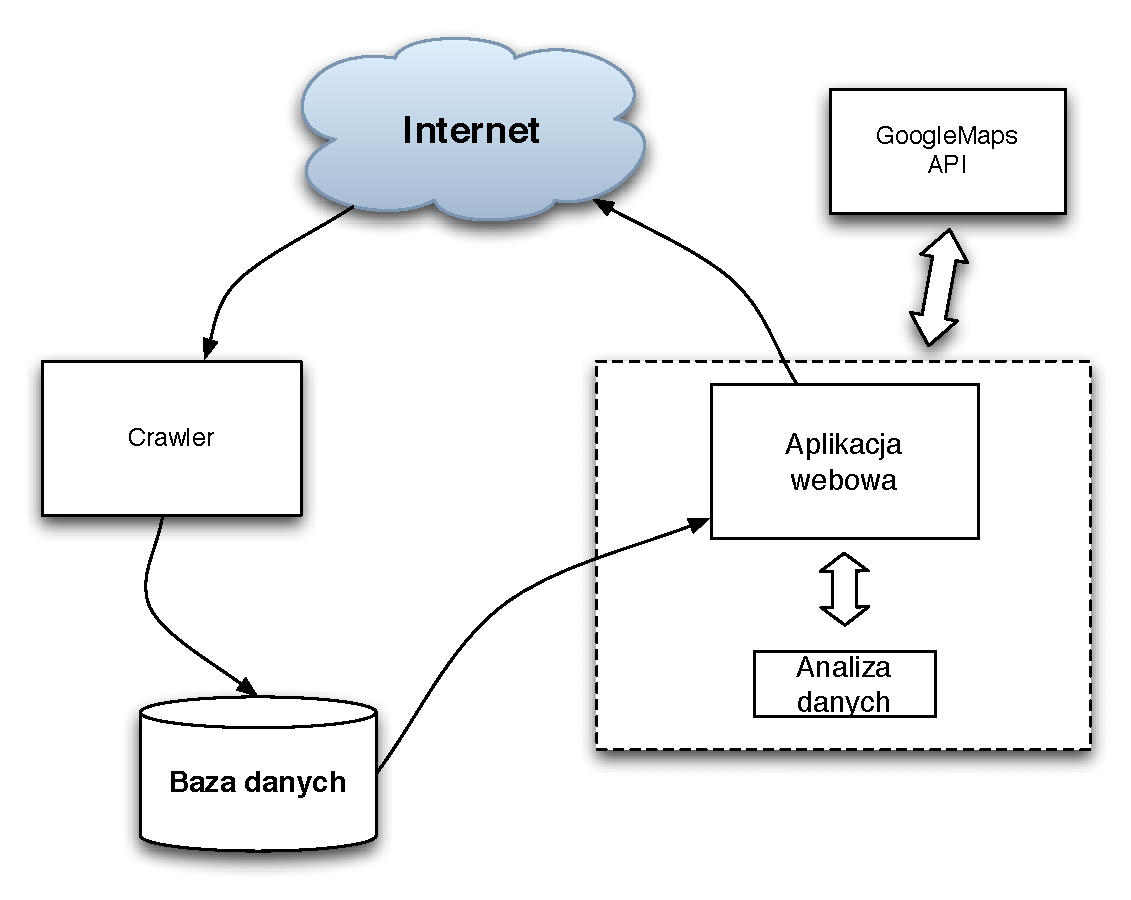
\includegraphics[width=35em]{images/data_flow_diagram.pdf}

\subsection{Entity Relationship Diagram}
Poniższy model danych nie jest dokładny, to znaczy tabele \texttt{resorts}
oraz \texttt{worldborders} są już stworzone natomiast pomiary zostaną dodane
dopiero po stworzeniu crawlera w związku z czym model może nie wyglądać tak samo.

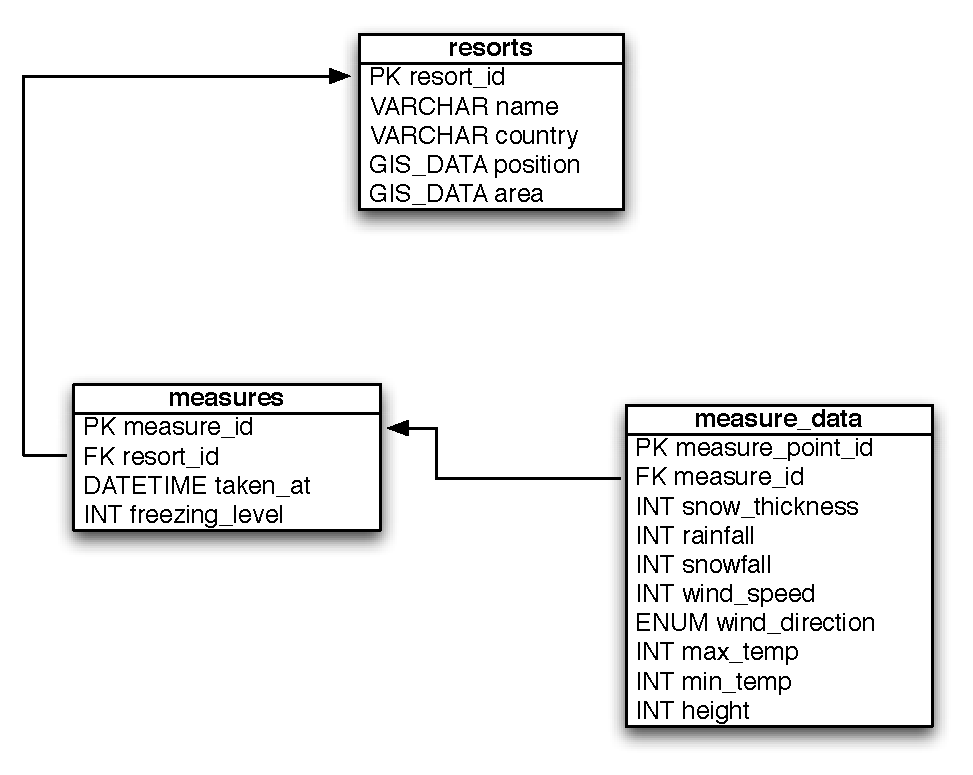
\includegraphics[width=35em]{images/erd_diagram.pdf}

\section{Aplikacja Django}
\subsection{Modele}
Wszystkie modele zawierają pole objects typu \texttt{models.GeoManager} który odpowiada za wspieranie zapytan Spatialowych.
Zdefiniowane w aplikacji modele to:
\begin{description}
\item[WorldBorders] odpowiada za przechowywanie granic państw. Pola modelu:
  \begin{description}
  \item[name] nazwa państwa
  \item[lat] szerokość geograficzna
  \item[lon] długość geograficzna
  \item[mpoly] typ \texttt{SDO\_GEOMETRY} przechowywujący \texttt{MultiPolygon} który
    definiuje granice państwa
  \end{description}
\item[Resorts] przechowuje ośrodki dla których posiadamy dane pogodowe. Pola:
  \begin{description}
    \item[name] nazwa miasta
    \item[position] dwuwymiarowa geometria \texttt{Point} przechowywująca długość i
      szerokość geograficzną miasta
  \end{description}
\item[MeasuresResorts] przechowuje dane dotyczące pomiarów w ośrodkach na różnych wysokościach.
  \begin{description}
    \item[resort] (FK) klucz obcy do tabeli Resorts, przechowuje id resortu którego dotyczy pomiar.
    \item[altitude] wysokośc n.p.m.
  \end{description}
\item[Measures] przechowuje poszczególne pomiary.
  \begin{description}
    \item[measure\_resort] (FK) klucz obcy do tabeli MeasuresResorts, przechowuje id ktorego konkretny pomiar dotyczy
    \item[taken\_at] typ \texttt{Datetime} przechowujący czas pomiaru.
    \item[max\_temp] maksymalna temperatura
    \item[min\_temp] minimalna temperatura
  \end{description}
\end{description}


\subsection{Metody}
\subsubsection{Wybranie obiektu z bazy}
\texttt{austria = WorldBorders.objects.filter(pk=Austria)[0]} \\
\texttt{first\_resort = Resorts.objects.all()[0]}

\subsubsection{Państwo, w którym leży resort}
\texttt{country = first\_resort.country()} \\
\texttt{print country.name \# => ``Austria``}

\subsubsection{Najbliższe resorty}
\texttt{resorts = first\_resort.within\_distance(30)} \\
\texttt{  \# => resorty w odległości 30km od danego (bez danego)}

\subsection{SQL}
\subsubsection{Stworzenie tabel}
Kluczowy dla projektu jest oczywiście typ \texttt{SDO\_GEOMETRY} który umożliwia wykonywanie
specyficznych zapytań geograficznych. Reszta pól to dodatkowe informacje na temat państwa/miasta.
\begin{verbatim}
CREATE TABLE "WORLD_WORLDBORDERS" (
    "NAME" NVARCHAR2(50) NOT NULL PRIMARY KEY,
    "LAT" DOUBLE PRECISION NOT NULL,
    "LON" DOUBLE PRECISION NOT NULL,
    "MPOLY" MDSYS.SDO_GEOMETRY NOT NULL
);
\end{verbatim}

\begin{verbatim}
CREATE TABLE "WORLD_RESORTS" (
    "NAME" NVARCHAR2(50) NOT NULL PRIMARY KEY,
    "POSITION" MDSYS.SDO_GEOMETRY NOT NULL
);
\end{verbatim}

Tabela pomiarów posiada dodatkowo klucz obcy do ośrodków aby pomiar można było zaklasyfikować do
danego ośrodka.
\begin{verbatim}
CREATE TABLE "WORLD_MEASURES" (
    "ID" NUMBER(11) NOT NULL PRIMARY KEY,
    "RESORT_ID" NUMBER(11) NOT NULL REFERENCES "WORLD_RESORTS" ("ID")
         DEFERRABLE INITIALLY DEFERRED,
    "TEMP" NUMBER(11) NOT NULL,
    "TAKEN_AT" DATE NOT NULL
);
\end{verbatim}

\paragraph{Ustawienia metryki}
Aby Oracle wiedział, jak wygląda metryka, należy poinformować go ustalając odpowiednie wartości graniczne
oraz dokładność dla kolumn Spatial. W tym wypadku informujemy, że kolumna \texttt{MPOLY} tabeli
\texttt{WORLD\_WORLDBORDERS} posiada zakres długości od -180 do 180 oraz szerokości od -90 do 90 z dokładnością
co 0.05.

\begin{verbatim}
INSERT INTO USER_SDO_GEOM_METADATA
   ("TABLE_NAME", "COLUMN_NAME", "DIMINFO", "SRID")
   VALUES (
    'world_worldborders',
    'mpoly',
    MDSYS.SDO_DIM_ARRAY(
      MDSYS.SDO_DIM_ELEMENT('LONG', -180.0, 180.0, 0.05),
      MDSYS.SDO_DIM_ELEMENT('LAT', -90.0, 90.0, 0.05)
    ),
    4326
  );
\end{verbatim}

\paragraph{Indeksy}
Aby zapytania mogły funkcjonować należy stworzyć indeksy na kolumnach spatial. Służy do tego celu polecenie
\begin{verbatim}
CREATE INDEX "WORLD_RESORTS_POSITION_ID"
ON "WORLD_RESORTS"("POSITION")
INDEXTYPE IS MDSYS.SPATIAL_INDEX;
\end{verbatim}

\paragraph{Sekwencje}
Warto wspomnieć, że część tabeli ma klucze główne liczbowe i aby nie przejmować się ich numerowaniem
stworzyć należy sekwencje. Do tego celu użyliśmy:
\texttt{CREATE SEQUENCE WORLD\_WORLDBORDERS\_SQ}
i analogiczne dla pozostałych tabel.

\subsubsection{Spatial queries}
\paragraph{Ośrodki w pobliżu danego ośrodka}
\begin{verbatim}
SELECT "WORLD_RESORTS"."ID", "WORLD_RESORTS"."NAME",
       SDO_UTIL.TO_WKTGEOMETRY("WORLD_RESORTS"."POSITION")
FROM "WORLD_RESORTS"
WHERE
    (SDO_WITHIN_DISTANCE("WORLD_RESORTS"."POSITION",
        SDO_GEOMETRY(POINT (10.7498 46.96297), 4326),
        \'distance=20000.0\') = \'TRUE\'
    AND NOT ("WORLD_RESORTS"."ID" = 832))
\end{verbatim}
\texttt{SDO\_WITHIN\_DISTANCE} to funkcja sprawdzająca czy geometria z pierwszego argumentu znajduje się w pewnej
odległości od geometrii drugiego. Jak widać drugą geometrię tworzymy przedstawiając dane geograficzne ośrodka
w postaci Well-Known Text: \texttt{POINT(10.749, 46.962)} pierwsza jest natomiast do tej postaci konwertowana
przez funkcję \texttt{TO\_WKTGEOMETRY}. Trzeci argument to odległość jako liczba metrów. Cała
funkcja zwraca true gdy warunek spełniony.

\paragraph{Państwo, w którym znajduje się ośrodek}
\begin{verbatim}
SELECT "WORLD_WORLDBORDERS"."ID", "WORLD_WORLDBORDERS"."NAME",
       "WORLD_WORLDBORDERS"."LAT", "WORLD_WORLDBORDERS"."LON",
       SDO_UTIL.TO_WKTGEOMETRY("WORLD_WORLDBORDERS"."MPOLY")
FROM "WORLD_WORLDBORDERS"
WHERE SDO_CONTAINS("WORLD_WORLDBORDERS"."MPOLY",
    SDO_GEOMETRY(POINT (10.7498 46.96297), 4326)) = \'TRUE\'
\end{verbatim}
W tym wypadku używamy funkcji \texttt{SDO\_CONTAINS} która zwraca prawdę, gdy druga gemoetria całkowicie zawiera pierwszą.
W naszym przypadku pierwszą geometrią jest wielobok przedstawiający granice państwa w tabeli państw natomiast druga to
punkt reprezentujący ośrodek. W ten sposób zwracamy wszystkie państwa których granice obejmująten punkt (w większości
przypadków będzie to jeden rekord).

\subsection{Integracja z GoogleMaps API}
API GoogleMaps jest w języku JavaScript. Wszystkie funkcje, ktorych używamy są zdefiniowane w widokach znajdujących
się w katalogu \texttt{world/templates}.

Głównym widokiem jest \texttt{layout.html} i on definiuje mapę i podstawowe funkcje wyświetlania resortów. Należy pamiętać,
że GoogleMaps działają tylko dla domeny, która została podana przy generowania klucza, dlatego jeśli domena będzie inna
(aktualnie \texttt{http://localhost:8000}) należy \href{http://code.google.com/apis/maps/signup.html}{wygenerować nowy klucz}
i zmienić widok \texttt{world/templates/layout.html}.

\subsubsection{Granice Austrii}
Granice wyświetlane są przez API KML-owe GoogleMaps. Reprezentację KML granic państwa mozna łatwo wyciągnąć z bazy
danych, jednak API nie pozwala na dynamiczne wyświetlanie plików KML i muszą one być dostępne publicznie w Internecie.
Z tego powodu wproowadzona jest redundancja danych: w pliku \texttt{world/templates/layout.html} znajduje się linia
\begin{verbatim}
var kml = new GGeoXml("http://student.agh.edu.pl/msq/austria.kml");
\end{verbatim}
która definiuje położenie pliku do wyświetlania. W razie potrzeby taki plik można wygenerować za pomocą następujących
poleceń:

\begin{verbatim}
python manage.py shell
> from world.models import WorldBorders
> austria = WorldBorders.objects.filter(pk="Austria")[0]
> print austria.mpoly.kml
\end{verbatim}

\subsection{Fikstury}
Dane do aplikacji mogą zostać ponownie załadowane do bazy (włącznie z uprzednim jej wyczyszczeniem). W plikach
\texttt{worldborders.fixtures} i \texttt{resorts.fixtures} znajdują się odpowiednie dane w prostym formacie tekstowym.
Aby załadować je do bazy należy wykonać następujące polecenia:
\begin{verbatim}
python manage.py shell
> from world import load
> load.load_fixtures()
> # lub load.load_worldborders()
> # lub load.load_resorts()
\end{verbatim}
Metoda \texttt{load.load\_fixtures()} czyści bazę i tworzy wszystkie fikstury natomiast metody \texttt{load.load\_worldborders()}
i \texttt{load.load\_resorts()} działają na poszczególnych tabelach.

\subsection{Wizualizacja danych}
W celu wizualizacji danych ściśle powiązanych z GIS wykorzystaliśmy dostępne w Oracle Spatial metody do pracy na wcześniej utworzonych oraz do tworzenia struktur GIS. Poza tym skorzystaliśmy z modułu PIL (Python Imaging Library) do tworzenia obrazów z otrzymanych danych typu WKT (Well-known text)

\subsection{Metody Oracle Spatial}
\subsubsection{SDO\_UTIL.TO\_WKTGEOMETRY}
Konwertuje zadany obiekt typu SDO\_GEOMETRY do typu WKT - well-known text.
\subsubsection{SDO\_GEOM.SDO\_BUFFER}
Tworzy wokół obiektu strefę buforową o zadanych parametrach (odległość oraz tolerancja)
\subsubsection{SDO\_GEOM.SDO\_CONVEXHULL}
Zwraca polygon wypukły oparty na elementach zadanego obiektu typu SDO\_GEOMETRY
\subsubsection{MDSYS.SDO\_GEOMETRY}
Tworzy strukturę geometryczną o zadanych parametrach (może to być np. polygon, kwadrat etc.)

\subsection{Konkretne zadania wizualizujące}
\subsubsection{Wizualizacja izoterm}
Do wizualizacji izoterm wykorzystaliśmy zapytania GeoDjango pozwalające na wybranie Resortów w określonej odległości od zadanego Resortu początkowego.

\begin{verbatim}
points_data = Resorts.objects.filter(
              position__dwithin=(self.position, distance_km),
              measuresresorts__measures__min_temp__lt=temperature
              ).unionagg().coords
\end{verbatim}

Następnie po przekonwertowaniu danych do odpowiedniego formatu korzystamy z nich przy generowaniu zapytania SQL.

\begin{verbatim}
SELECT SDO_UTIL.TO_WKTGEOMETRY(
 SDO_GEOM.SDO_BUFFER(
  SDO_GEOM.SDO_BUFFER(
   SDO_GEOM.SDO_CONVEXHULL(
    MDSYS.SDO_GEOMETRY(
     2003,
     4326,
     NULL,
     SDO_ELEM_INFO_ARRAY(1, 2003, 1),
     SDO_ORDINATE_ARRAY(%s)),
    50),
   100, 50, 'unit=m'),
  20, 50, 'unit=m')
 ) FROM WORLD_WORLDBORDERS;" % points_str
\end{verbatim}

Zwracane dane to (w przypadku pomyślnego wyszukania odpowiednich danych resortów, POLYGON w formacie WKT (well-known text). Następnie polygon przetwarzany jest przez odpowiednie metody w PIL (python imaging library) i wraz z danymi GIS danego kraju tworzony jest obraz przedstawiający izotermę następującej postaci:

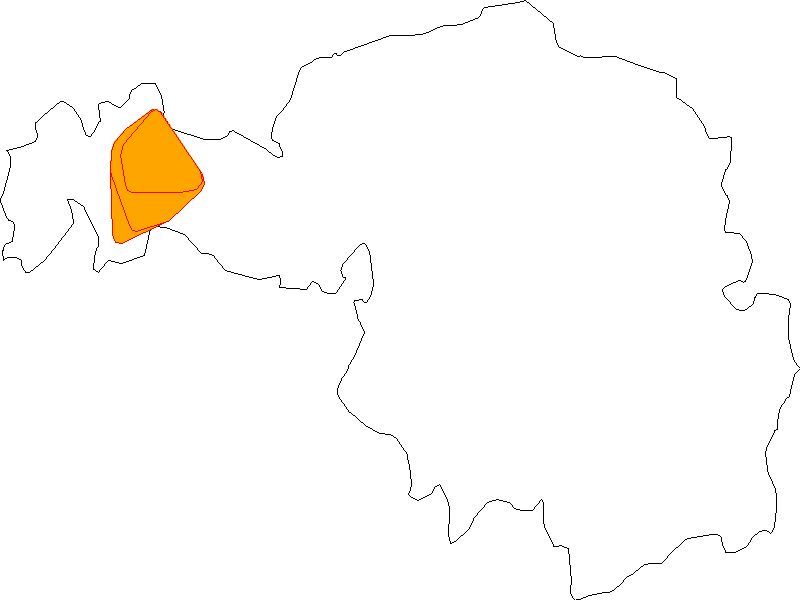
\includegraphics[width=35em]{images/isotherm.png}

\section{Crawler}
Crawler jest napisany w języku Ruby i służy do pobierania danych ze strony
\\\url{http://www.snow-forecast.com}.
Docelowo będzie to prosty skrypt oparty o metodologię \emph{Extract--Transform--Load}.
\subsection{Extract}
\begin{itemize}
\item uruchamiamy skrypt z parametrem adresu strony (w zasadzie chodzi o wybrany szczyt)
\item skrypt analizuje stronę za pomocą parsera HTML+XML Nokogiri
\item dane zapisywane są w prostej postaci w tablicy
\item skrypt znajduje link do danych z poprzedniego okresu, odwiedza go i powtarza proces
\end{itemize}
Dane zapisywane są przez
\begin{verbatim}
file = File.open(filename, "w")
file.write(Marshal.dump(data))
\end{verbatim}
Aby je odczytać wystarczy
\begin{verbatim}
data = Marshal.load(File.read(filename))
\end{verbatim}

\section{Plan prac}
Plan jest ułożony malejąco względem priorytetów.
\subsection{Crawler}
\begin{itemize}
  \item część \emph{Transform} przerabiające surowe dane na potrzeby aplikacji
  \item część \emph{Load} tworząca SQL-e i wykonująca je w kontekście bazy
\end{itemize}

\subsection{Import danych}
\begin{itemize}
  \item utworzenie odpowiednich tabel do przetrzymywania danych, utworzenie relacji między tabelami
  \item zmapowanie tabel w modelach Django
  \item ustalenie formatu danych oraz ich konwersja do formatu odpowiadającego modelowi w bazie danych
  \item zaimportowanie danych do bazy danych
  \item utworzenie części aplikacji odpowiedzialnej za aktualizację zbieranych danych
\end{itemize}

\subsection{Analiza danych}
\begin{itemize}
  \item umożliwienie wyświetlania prognozowanych danych dla resortów, dla których istnieją pobrane dane
        (podpierając się GIS)
  \item implementacja systemu 'przewidującego' pogodę na podstawie poprzednich danych (na życzenie lub w
        sytuacji gdy dane prognozowane nie są dostępne)
  \item porównywanie danych z różnych ośrodków oraz przedstawienie raportów
  \item dobieranie najoptymalniejszego resortu spośród dostępnych raportów na bazie preferencji użytkownika
  \item możliwość zacieśnienia przeszukiwanych/porównywanych resortów tylko i wyłącznie do określonego regionu
  \item dobór ośrodka na podstawie aktualnej pozycji użytkownika (np. odległość od domu/odległość od ośrodka
        w którym użytkownik znajduje się aktualnie, a np. nie jest zadowolony)
\end{itemize}

\subsection{Wizualizacja danych}
\begin{itemize}
  \item prezentowanie aktualnych danych w postaci różnego rodzaju wykresów (np. stosunek świeżego śniegu
        do grubości pokrywy śnieżnej, prezentacja temperatur na różnych wysokościach)
  \item generowanie wykresów na podstawie danych historycznych (np. temperatury z ostatniego tygodnia)
  \item wizualizacja porównawcza różnych ośrodków (prezentacja różnic w temperaturze, wietrze i śniegu dla
        dwóch lub więcej ośrodków)
  \item przedyskutowanie dalszych możliwości wizualizacji danych
  \item wizualizacja danych prognozowanych za pomocą Google Maps API
\end{itemize}

\subsection{Dodatkowe}
\begin{itemize}
  \item wyszukanie serwisów prognozujących pogodę dla konkretnych regionów w Austrii (dostosowanie crawlera)
  \item implementacja wyszukiwania ośrodków
  \item utworzenie możliwości deklarowania preferencji przez użytkownika oraz ich zapisywanie
  \item możliwośc wyszukiwania bazującego na preferencjach użytkownika, poszerzenie systemu wyszukiwania
  \item próba wykorzystania Google Maps API do prezentowania dokładniejszej odległości danego ośrodka od
        użytkownika (na podstawie jego aktualnej pozycji np. w preferencjach)
\end{itemize}

\section{Linki}
\begin{description}
  \item[Źródła (repozytorium Git)] \url{http://github.com/michalbugno/projekt-oszbd/}
  \item[Projekt Django] \url{http://www.djangoproject.com/}
  \item[Projekt GeoDjango] \url{http://geodjango.org/}
  \item[API GoogleMaps] \url{http://code.google.com/apis/maps/documentation/}
  \item[System kontroli wersji Git] \url{http://git-scm.com/}
  \item[Python] \url{http://www.python.org/}
  \item[Ruby] \url{http://www.ruby-lang.org/}
\end{description}

\end{document}
